% =============================================================================
% COPYRIGHT AND DISCLAIMER
% =============================================================================
% This file is provided as a convenience template for competition participants.
% By using it, you accept full responsibility for compliance with all applicable
% copyright, licensing, and usage rules of the Association for Computing
% Machinery (ACM) and of any LaTeX packages you load (including, without
% limitation, the "acmart" document class and related ACM materials).
%
% Consult ACM's official publication, template, and copyright policies before
% using this setup for any purpose other than this competition. Do not assume
% that this template may be reused, redistributed, or submitted elsewhere
% without independently verifying ACM's current rules.
%
% Use of the "acmart" class, the "sigconf" option, or ACM-style formatting in
% this template does NOT mean that this report, this competition, its organizers,
% or any resulting PDF is sponsored, endorsed, affiliated with, or published by
% ACM. ACM trademarks and branding remain the property of ACM.
%
% Template packages live in preamble.tex.
% Citations live in main.bib. Edit this file with your paper content.
% =============================================================================

\documentclass[sigconf]{acmart}
\input{preamble}
\usepackage{tikz}
\usetikzlibrary{positioning,arrows.meta}

% Guide styling: \guideStyletrue = show gray italic hints; \guideStylefalse = omit them
% \guideStyletrue
\guideStylefalse

\begin{document}

\title{Two Detectors, One Jury}  % Replace this with your title
\subtitle{A Solution to the Solar Filament Segmentation Challenge 2026} % DO NOT CHANGE


\author{Jhonatan Venegas}
\affiliation{%
  \institution{Independent participant}
  \city{Quer\'etaro}
  \country{Mexico}
}
\email{jhonatanvenegasjharol@gmail.com}   % <- Replace with your own email

\begin{abstract}
    This report describes our solution to the Solar Filament Segmentation Challenge~2026, a Kaggle competition on automatic segmentation of solar filaments in GONG H-$\alpha$ observations. Two YOLO11-seg instance detectors, one fed with the plain image and one with three processed views of it, propose filaments; a U-Net refiner redraws each proposal at full resolution; and a two-of-two jury keeps only what both detectors see. On a fixed local exam of 121 training images the model reaches a Panoptic Quality of 0.461 (95\% bootstrap interval 0.444--0.479), against 0.340 when one expert is scored against another, and 0.39 on the public leaderboard. Its matched masks overlap the experts' with a mean IoU of 0.68, higher than two experts reach with each other (0.64). Most of the remaining error lies in small, faint filaments on which the experts themselves disagree.
\end{abstract}

\maketitle

% ==================================== %
%              INTRODUCTION            %
% ==================================== %
\section{Introduction}
    This report goes over the details of our submitted solution to the Solar Filament Segmentation Challenge~2026 \cite{filament-segmentation-2026}. The challenge, launched on July~10,~2026, is organized by the Earth-Space AI Research (ESAIR) Lab\footnote{\href{https://www.esairlab.com/home}{www.esairlab.com/}}. This challenge utilizes the MAGFiLO dataset for evaluation of the segmentation algorithms \cite{ahmadzadeh2024dataset}. I entered it to measure my ability to solve a real problem that matters beyond the competition. The code, the weights of the final model and a notebook that reproduces the submission are at \url{https://github.com/Cryptokepler/filamentos-solares-2026}; every experiment, with its expected result written before running it and the measured result after, is in \texttt{docs/experimentos.md}.

    Our main contributions are: (i) an instance-detection pipeline that segments filaments better than one expert matches another; (ii) a jury of two detectors that look at the image differently; and (iii) an analysis showing that the remaining error is dominated by disagreement between annotators rather than by what the model can see.


% ==================================== %
%              METHODOLOGY             %
% ==================================== %
\section{Methodology}\label{sec:methodology}

\begin{figure*}[t]
\centering
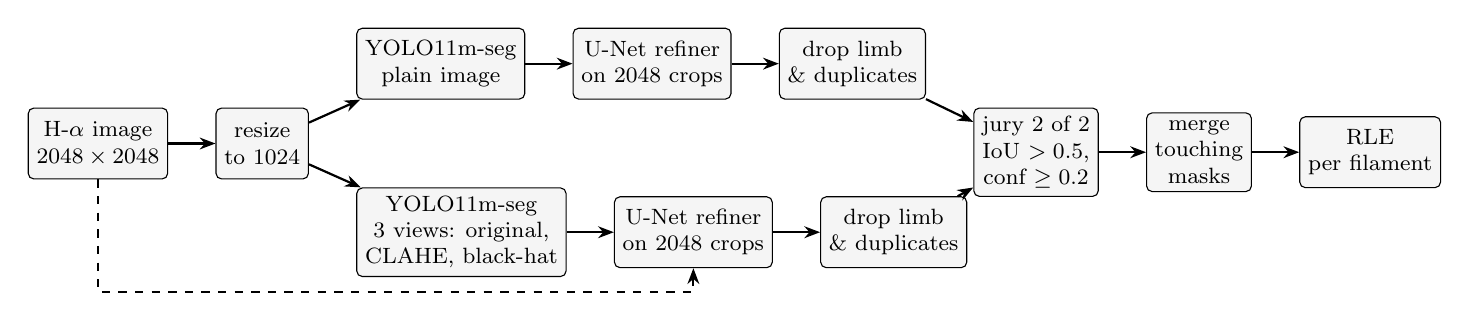
\begin{tikzpicture}[
  box/.style={draw, rounded corners=2pt, align=center, font=\footnotesize, minimum height=9mm, inner sep=3pt, fill=gray!8},
  arr/.style={-{Stealth[length=2mm]}, thick}]
\node[box] (img) {H-$\alpha$ image\\$2048\times2048$};
\node[box, right=6mm of img] (res) {resize\\to 1024};
\node[box, above right=1mm and 6mm of res] (y5) {YOLO11m-seg\\plain image};
\node[box, below right=1mm and 6mm of res] (y7) {YOLO11m-seg\\3 views: original,\\CLAHE, black-hat};
\node[box, right=6mm of y5] (r5) {U-Net refiner\\on 2048 crops};
\node[box, right=6mm of y7] (r7) {U-Net refiner\\on 2048 crops};
\node[box, right=6mm of r5] (c5) {drop limb\\\& duplicates};
\node[box, right=6mm of r7] (c7) {drop limb\\\& duplicates};
\node[box, below right=1mm and 6mm of c5] (jury) {jury 2 of 2\\IoU $>0.5$,\\conf $\ge0.2$};
\node[box, right=6mm of jury] (merge) {merge\\touching\\masks};
\node[box, right=6mm of merge] (out) {RLE\\per filament};
\draw[arr] (img) -- (res); \draw[arr] (res) -- (y5); \draw[arr] (res) -- (y7);
\draw[arr] (y5) -- (r5); \draw[arr] (y7) -- (r7); \draw[arr] (r5) -- (c5); \draw[arr] (r7) -- (c7);
\draw[arr] (c5) -- (jury); \draw[arr] (c7) -- (jury); \draw[arr] (jury) -- (merge); \draw[arr] (merge) -- (out);
\draw[arr, dashed] (img.south) |- ([yshift=-3mm]r7.south) -- (r7.south);
\end{tikzpicture}
\caption{End-to-end pipeline of the final model. The refiner reads crops of the original $2048\times2048$ image (dashed arrow). Code: \texttt{filamentos/final.py}.}
\label{fig:pipeline}
\end{figure*}

\subsection{Data split and training examples}
The 707 training images were split once, before any experiment, into 586 for training and 121 for a local exam ($\mathrm{md5}(\text{file name}) \bmod 100 < 15$); the exam images were never used to train any model; they only served to pick each detector's best epoch and to compare rounds. 296 images carry two or three expert annotations. Instead of fusing them, every expert's annotation of an image is a separate training example, so the model sees the full range of expert judgement. Images are grayscale JPEGs; we use them without calibration, only resized.

\subsection{Detectors}
We use YOLO11m-seg \cite{yolo11} (Ultralytics, COCO-pretrained), an instance-segmentation detector that predicts a box, a confidence and a mask prototype combination per object. We chose instance detection over semantic segmentation because the metric scores each filament as an object: in our first round a U-Net with connected components split filaments and merged neighbours (93 split, 27 merged on the exam), while a detector proposes whole filaments (18 and 43). Both detectors are trained at 1024~px for up to 2.5~h on one T4 GPU (batch 6, flips, brightness jitter, mosaic, cosine schedule; best epoch on the exam's mAP).

The first detector sees the plain image. The second sees three views of it, one per colour channel: the original; local contrast (CLAHE, tiles of 64 px); and a black-hat map (morphological closing with a 25~px disk minus the image) that keeps only what is darker than its surroundings and thin, removing the limb darkening. The idea of ``removing the pigment'' comes from how models work: they do not see the image as we do but through abstract patterns, so we looked for views that make the patterns and irregularities we care about easier to pick up. Each detector proposes every object with confidence $\ge 0.1$.

\subsection{Refiner}
Detector masks at 1024~px are coarse at the edges. A U-Net \cite{unet} with a ResNet-18 encoder (ImageNet-pretrained, \texttt{segmentation-models-pytorch}) redraws each proposal: a square crop of $1.8\times$ the proposal's size is cut from the $2048$~px image, resized to $256$~px, segmented (four flips averaged, threshold 0.5) and pasted back. Only the connected component that touches the detector's mask is kept, so a neighbouring filament inside the crop is not swallowed. The refiner was trained on expert masks with jittered crops (margin 1.5--2.2, shifts up to 10\%) so it does not depend on perfect boxes.

\subsection{Post-processing and jury}
For each detector we drop proposals whose mean distance to the disk centre exceeds $0.95\,R_\odot$ (limb artefacts) and near-duplicates (IoU $>0.5$ with a more confident proposal). Proposals of the two detectors that overlap with IoU $>0.5$ form a \emph{case}; a case is kept only if both detectors see it with confidence $\ge 0.2$, and its mask is the most confident refined mask. Finally, kept masks that touch are merged, so no pixel belongs to two filaments. Inference uses only the test image (no metadata, no neighbouring frames) and takes about 14~s per image on a 4-core CPU.

\begin{figure}[t]
\centering
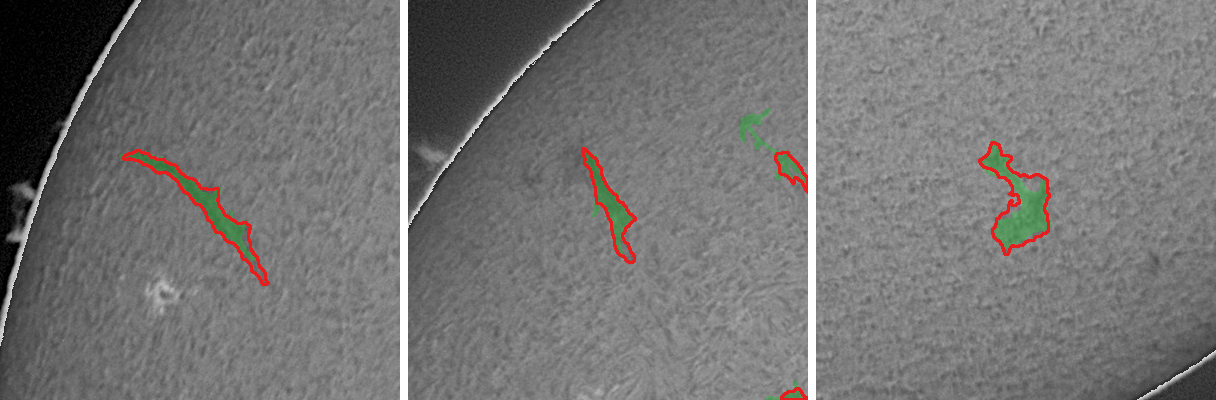
\includegraphics[width=\columnwidth]{examples.png}
\caption{Exam examples (crops at full resolution). Green: one expert's annotation; red outline: our final model.}
\label{fig:examples}
\end{figure}


% ==================================== %
%              EVALUATION              %
% ==================================== %
\section{Evaluation}\label{sec:evaluation}

\subsection{Strategy}
We score with the competition's Panoptic Quality, $\mathrm{PQ} = \mathrm{SQ}\times\mathrm{RQ}$, where a prediction matches an annotation when IoU $>0.5$, SQ is the mean IoU of matches and $\mathrm{RQ}=\frac{TP}{TP+\frac12FP+\frac12FN}$. Each expert's annotation of an exam image is scored separately and the counts are pooled. During the competition the public leaderboard was unreliable (empty masks and leaked annotations scored above 0.55), so we never tuned on it: every decision was taken on the local exam. Its uncertainty comes from a bootstrap over the 121 images (2{,}000 resamples). Across rounds the exam predicted the direction of the Kaggle score with an offset of about $-0.07$. As a human reference, scoring one expert against another on the 296 multi-expert images gives PQ $=0.340$ and SQ $=0.64$.

\subsection{Results}
Table~\ref{tab:rounds} lists the rounds that changed the model. The large step was moving from semantic segmentation to detection plus refinement ($+0.06$); YOLO and the jury then added about $0.01$ each. The jury works because the two detectors fail in different places: a jury of identical YOLOs trained on 25--100\% of the data gave no gain (0.454--0.458).

\begin{table}[t]
\caption{Local exam (121 images, all experts pooled). TP: matched, FP: invented, FN: missed. $\pm$: bootstrap standard deviation.}
\label{tab:rounds}
\centering\small
\begin{tabular}{@{}lccc@{}}
\toprule
Model & PQ & TP / FP / FN & Kaggle \\
\midrule
Expert vs.\ expert & 0.340 & -- & -- \\
Classical (dark regions) & 0.098 & -- & -- \\
U-Net + rules & 0.384 & 826 / 648 / 541 & 0.34 \\
Mask R-CNN + refiner & 0.441 & 820 / 350 / 547 & 0.38 \\
YOLO plain + refiner & 0.456 & 878 / 381 / 489 & -- \\
YOLO 3 views + refiner & 0.456 & 871 / 366 / 496 & -- \\
\textbf{Final: jury of both} & \textbf{0.461 $\pm$ 0.009} & 894 / 379 / 473 & \textbf{0.39} \\
\bottomrule
\end{tabular}
\end{table}

\textbf{Mask quality.} The final model's matched masks have a mean IoU of 0.68 (Dice 0.81); the median IoU is 0.68 and 90\% of matches exceed 0.56. Fragmentation is rare: 18 annotated filaments are covered by two or more of our masks (one-to-many) and 41 of our masks cover two or more annotations (many-to-one). Thin structures (barbs, tails) were measured by morphological opening: of the expert's parts thinner than 9~px we cover 65.5\%, another expert covers 66.9\%. Our masks are smoother (thin part 7\% of the area vs.\ 14\%) and miss some tails at the ends.

\textbf{Measured negative results.} Test-time flips ($-0.008$); a small-filament specialist at 2048~px (finds 88 more, invents $\sim$170); more images of the same kind (learning curve 0.428 / 0.447 / 0.440 / 0.453 at 25 / 50 / 75 / 100\%); rule-based and learned judges on crops and features (0.444); a third detector on a Frangi vesselness view; higher refiner thresholds; growing tails along dark ridges ($-0.001$ to $-0.017$); and joining fragments or removing small masks.

\subsection{Strengths, weaknesses and improvement}
The model's strength is shape: once a filament is found, its outline agrees with an expert more than another expert's does, and it rarely splits or merges. Its weakness is small, faint filaments. Of the remaining errors of the plain YOLO model, the largest shares are filaments we ``invented'' that another expert did draw (161), misses drawn by only one expert (182) and errors on images with a single annotator (302); errors that are clearly ours add up to about 280, worth at most $+0.05$. 85\% of misses are smaller than 3{,}000~px, exactly where experts agree least: under 330~px another expert draws a matching filament only 41\% of the time. At 1024~px these filaments are still $\sim$6~px wide, so resolution is not the limit. Predicting the union of all experts would score 0.658 and copying a single expert 0.605: a model trained on all experts learns their average judgement. Promising directions are pretraining on unlabeled H-$\alpha$ images and training-only magnetograms, which mark the polarity inversion lines filaments lie on.

\textbf{A personal note on expert disagreement.} What surprised me most was the clash between experts. Scored against a single expert a model can look very good; other experts have a different point of view, and the average falls. It also taught me about human cognitive biases and why information has to be contrasted, which is what I tried to build into this system, designed with artificial intelligence and my own judgement: two models must agree before a filament is accepted. I do not see the disagreement as a flaw of the dataset. People learn in different ways and do not all see the same thing; several points of view cover more angles, even blind spots, and from there an agreement, or a disagreement, can be reached.


% ==================================== %
%            ACKNOWLEDGMENT            %
% ==================================== %
\section{Acknowledgment}\label{sec:acknowledgment}
    % Do not change
    The organization of the Filament Segmentation Challenge 2026 is partially supported by the U.S. National Science Foundation (NSF) under Grant No. 2209912 and 2433781, directorate for Computer and Information Science and Engineering (CSE), and Office of Advanced Cyberinfrastructure (OAC), and Grant No. 2511630, AST Division Of Astronomical Sciences and MPS Directorate for Mathematical and Physical Sciences.

    The Filament Segmentation Challenge 2026 is sponsored by the U.S. National Science Foundation (NSF) National Solar Observatory (NSO).

    This work utilizes GONG data obtained by the NSO Integrated Synoptic Program, managed by the National Solar Observatory, which is operated by the Association of Universities for Research in Astronomy (AURA), Inc. under a cooperative agreement with the National Science Foundation and with contribution from the National Oceanic and Atmospheric Administration. The GONG network of instruments is hosted by the Big Bear Solar Observatory, High Altitude Observatory, Learmonth Solar Observatory, Udaipur Solar Observatory, Instituto de Astrofísica de Canarias, and Cerro Tololo Interamerican Observatory.

\bibliographystyle{ACM-Reference-Format}
\bibliography{main}

\end{document}
